\documentclass[convert]{standalone}
\usepackage[utf8]{inputenc}
\usepackage[T1]{fontenc}
\usepackage{amsmath}
\usepackage{amssymb}
\usepackage{tikz}
\usepackage{color}

\definecolor{draculaPurple}{RGB}{189,147,249}
\definecolor{draculaCyan}{RGB}{139,233,253}
\definecolor{draculaForeground}{RGB}{248,248,248}

\newcommand{\firstcircle}{(0,0) circle (1)}
\newcommand{\secondcircle}{(1,0) circle (1)}

\tikzset{reverseclip/.style={overlay,insert path={(-16383.99999pt,-16383.99999pt) rectangle (16383.99999pt,16383.99999pt)}}}

\begin{document}
	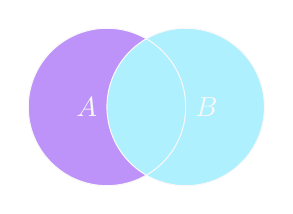
\begin{tikzpicture}[fill=draculaCyan, text=draculaForeground, draw=draculaForeground]
		\fill[opacity=0.7] \firstcircle;
%		\fill[opacity=0.7] \secondcircle;
		
		\begin{scope}
			\clip[reverseclip] \secondcircle;
			\fill[draculaPurple] \firstcircle;
		\end{scope}
	
		\begin{scope}
			\clip[reverseclip] \firstcircle;
			\fill[opacity=0.7] \secondcircle;
%			\fill[draculaPurple] \secondcircle;
		\end{scope}
	
		\draw \firstcircle node [left] {$A$};
		\draw \secondcircle node [right] {$B$};
	\end{tikzpicture}
\end{document}